\documentclass{article}
\usepackage[utf8]{inputenc}
\usepackage[greek,english]{babel}
\usepackage{alphabeta}
\usepackage{fancyhdr}
\usepackage{listings}
\usepackage{mathtools}
\usepackage{xcolor}
\usepackage{biblatex}
\usepackage[left=1cm,right=1cm]{geometry}

\lstset {
        basicstyle=\ttfamily,
        columns=fullflexible,
        breaklines=true,
        keepspaces=true,
	showstringspaces=false
}

\title{Εργαστήριο Παράλληλων Συστημάτων - Εργασία 1}
\author{Χρήστος Μαργιώλης}
\date{Δεκέμβριος 2022}

\begin{document}

\begin{titlepage}
        \maketitle
\end{titlepage}

\renewcommand{\contentsname}{Περιεχόμενα}
\tableofcontents
\pagebreak

\section{Κώδικας}

Ο κώδικας έχει σχόλια μόνο στα σημεία που θεώρησα ότι μπορεί να προκύψει κάποιο
«μπέρδεμα».

\lstinputlisting[language=C]{ex1.c}

\section{Προβλήματα}

Δεν κατάφερα να υλοποιήσω τον υπολογισμό του ελάχιστο με χρήση αλγορίθμου
δυαδικού δέντρου (ερώτημα d2.2).

\section{Βοηθητικό script}

\lstinputlisting[language=sh]{randinput}

Το script \lstinline{randinput} (δεν τρέχει σε Windows) δέχεται ως είσοδο τον
αριθμό των νημάτων, καθώς και το $N$. Στην συνέχεια τυπώνει (με την
συγκεκριμένη σειρά) τον αριθμό των νημάτων, το $N$, και $N$ τυχαίους αριθμούς.
Αυτό είναι χρήσιμο στο να μπορούμε να κάνουμε δοκιμές με διαφορετικά δεδομένα
(ειδικά για μεγάλες τιμές $N$) χωρίς να πρέπει να δώσουμε τα δεδομένα
χειροκίνητα.

Η χρήση του script έχει ως εξής:

\begin{lstlisting}
usage: randinput nthreads N
\end{lstlisting}

Παρακάτω φαίνεται μία ενδεικτική χρήση:

\begin{lstlisting}
$ ./randinput 2 3
2
3
8
0
1
5
1
2
0
4
8
\end{lstlisting}

'Αρα έχουμε 2 νήματα, έναν πίνακα $3x3$, τα στοιχεία του οποίου είναι:
\[[[8, 0, 1], [5, 1, 2], [0, 4, 8]]\]

Τώρα, μπορούμε να διοχετεύσουμε την έξοδο του script σε ένα αρχείο και να το
δώσουμε ως είσοδο στο κύριο πρόγραμμα:

\begin{lstlisting}
./randinput 2 3 > input.txt
\end{lstlisting}

\section{Ενδεικτικά τρεξίματα}

\textit{Σημειώνεται ότι το πρόγραμμα τρέχει κανονικά και χωρίς αρχείο για είσοδο.}

Για 2 threads και $A = 4x4$:

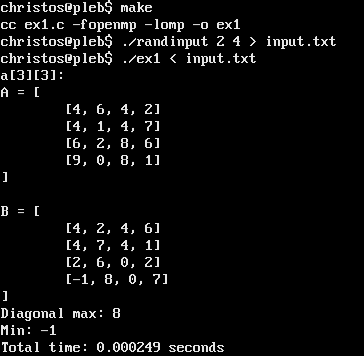
\includegraphics[width=\textwidth]{res/run1.png} \\

Για 4 threads και $A = 10x10$:

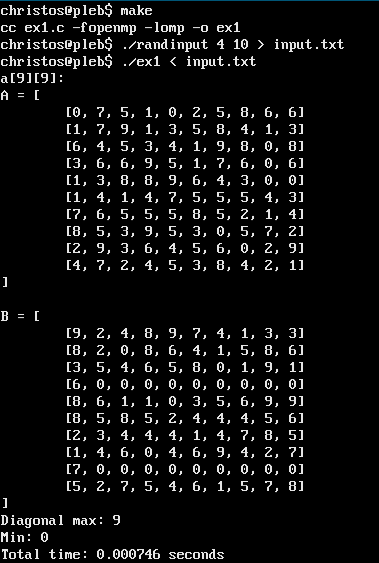
\includegraphics{res/run2.png} \\

Για 3 threads και $A = 100x100$. Παρατηρούμε ότι το συγκεκριμένο τρέξιμο
είχε δεδομένα τέτοια ώστε να μην πληρείται η προϋπόθεση του να είναι ο πίνακας
αυστηρά διαγώνια δεσπόζων:

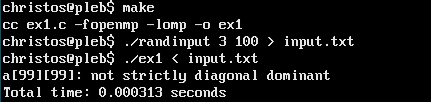
\includegraphics[width=\textwidth]{res/run3.png} \\

Στα παρακάτω τρεξίματα ο πίνακας θα είναι $1000x1000$, θα έχει τα ίδια
στοιχεία, αλλά κάθε τρέξιμο θα έχει διαφορετικό αριθμό threads, ωστέ να
παρατηρήσουμε τις διαφορές στην ταχύτητα εκτέλεσης του προγράμματος ανάλογα με
τον αριθμό των threads.

Παρατηρούμε ότι όταν τα threads είναι περισσότερα από 1, η ταχύτητα εκτέλεσης
σχεδόν υποδιπλασιάζεται.

Για 1 thread:


\includegraphics[width=\textwidth]{res/run4.png} \\

Για 2 threads:


\includegraphics[width=\textwidth]{res/run5.png} \\

Για 3 threads:


\includegraphics[width=\textwidth]{res/run6.png} \\

Για 4 threads:


\includegraphics[width=\textwidth]{res/run7.png} \\

\end{document}
